\section{Discussion}

%Content dump for weighted form

% It is intuitive that the measure of bag of properties will always give higher (or at least, equal) amount of wealth compared to the measure of set. Set of property will have an upper bound of number of unique property, while bag of property does not have any upper bound. Moreover, using bag of properties, a large number of triples having the same property may inflate the wealth substantially--though this is not necessarily a problem nor an advantage.

Set of properties might be more suitable if the main concern is the presence of properties, instead of the abundance of information it contains. We will take \textit{WilliamShakespeare} (Q692) in Wikidata as an example. It is reasonable if property like  \textit{date of birth} (P569) to be treated using set of properties, but for a well-known playwright and poet, we shall expect the property \textit{notable work} (P800) to incorporate all or most of his well-known works. If only few works registered in \(G\) despite he has dozens of works, then we might conclude the entity is poor. For this case, treating the property using the notion of set is not preferable because it will fail to capture the aforementioned poor condition, while blatantly using bag of properties might skew the wealth amount.

Another phenomena that should be considered is that an entity might have several occurrences of the same property, but this property might just be 'trivial'. This is similar to a document having a lot of 'the' or 'a' (stopwords). An entity might have just a single occurrence of a property, but it is a non-trivial one. Perhapse, the property is a highly relevant one for the entity's class. For example, \textit{timePeriod} for \textit{William Shakespeare} will be a highly relevant one for prominent poets. However, the property \textit{sibling} might not be too relevant for Shakespeare's career.

Due to this, the notion of (non-)uniqueness can be extended to a weighted form. The weight is given independently for each property and can be defined in such a way that is most appropriate for the nature of the property. Example of definition for weight are threshold function and inverse of median.

Let \(w_i\) be the weight of property \(p_i\) in graph \(G\). Let \(N_{bag}(S,G,p_i)\) be a set that comprises all pair  \((o,p_i)\), that is, property \(p_i\) and an object that is connected to \(S\). Then \(W_{weighted}(S, G)\) is the sum of \(N_{bag}(S,G,p_i)\) multiplied by the associated weight \(h_i\).

\textit{how can we formalize wi to be the function of set(amount of pi in class C in G)??}
\[
    \forall p_i, h_i = f(....)
\]
\[
    N_{bag}(S,G,p_i) = \{(p_i, o) | (S, p_i, o) \in G\}
\]
\[
    W_{weighted}(S, G) = \sum_i |N_{bag}(S,G,p_i)| * h_i
\]

\autoref{fig:wealth-weighted} shows how the notion of weighted wealth can be calculated. Let's define \(h_1 = 1/median\) and \(h_2 = 1\). For property \(p_1\), \({1, 2, 2, 4}\) list all sorted amount of information contributed from \(p_1\) in each individual entity from \(S_1\) to \(S_4\), from which we get \(h_1 = 1/median = 1/2\). With the above definition, \(W_{weighted}(S1, G) = 2\), \(W_{weighted}(S2, G) = 2\), \(W_{weighted}(S3, G) = 3.5\), \(W_{weighted}(S1, G) = 1.5\).

=====> OR (alternative of weighted, or generalized form of Wealth based on the (non-)uniqueness of individual properties)

=====> \(T_i\) is a multiset \(T_i = ... \) -> isinya list semua kontribusi wealth dari property \(p_i\) pada seluruh entity \(S\) pada class \(C\) di graph \(G\) -> keuntungannya disini kita jadi bisa punya fungsi konstan, sehingga bisa catter definisi set, bag, dan weighted secara bersamaan.

Let \(S_1\), \(S_2\), ... \(S_m\) be \(m\) distinct entities in graph \(G\), which all of them collectively create a class \(C\). Let \(N_{bag}(S_j,G,p_i)\) be a set that comprises all pair of a particular property \(p_i\) and object, \((p_i,o)\), that is connected to \(S_j\). We define \(T_{C,i}\) a multiset consisted of the number of non-unique properties of all entities of \(C\) contributed from property \(p_i\), i.e., cardinality of \(N_{bag}(S_j,G,p_i)\). Let \(f\) be a multivariate function with 2 arguments: \(T_{C,i}\) and \(N_{bag}(S_j,G,p_i)\). \(w_{j,i}\) is the amount of wealth of \(S_j\) attributed from property \(p_i\), which is calculated by function \(f\). Then \(W_{}(S_j, G)\) is the sum of \(w_{j,i}\).


\[
    N_{bag}(S_j,G,p_i) = \{(p_i,o) | (S_j, p_i, o) \in G\}
\]
\[
    T_{C,i} = \{|N_{bag}(S_j,G,p_i)| | S_j \in C\}
\]
\[
    w_{j,i} = f(T_{C,i}, |N_{bag}(S_j,G,p_i)|)
\]
\[
    W_{}(S_j, G) = \sum_i w_{j,i}
\]

\begin{figure}
    \centering
    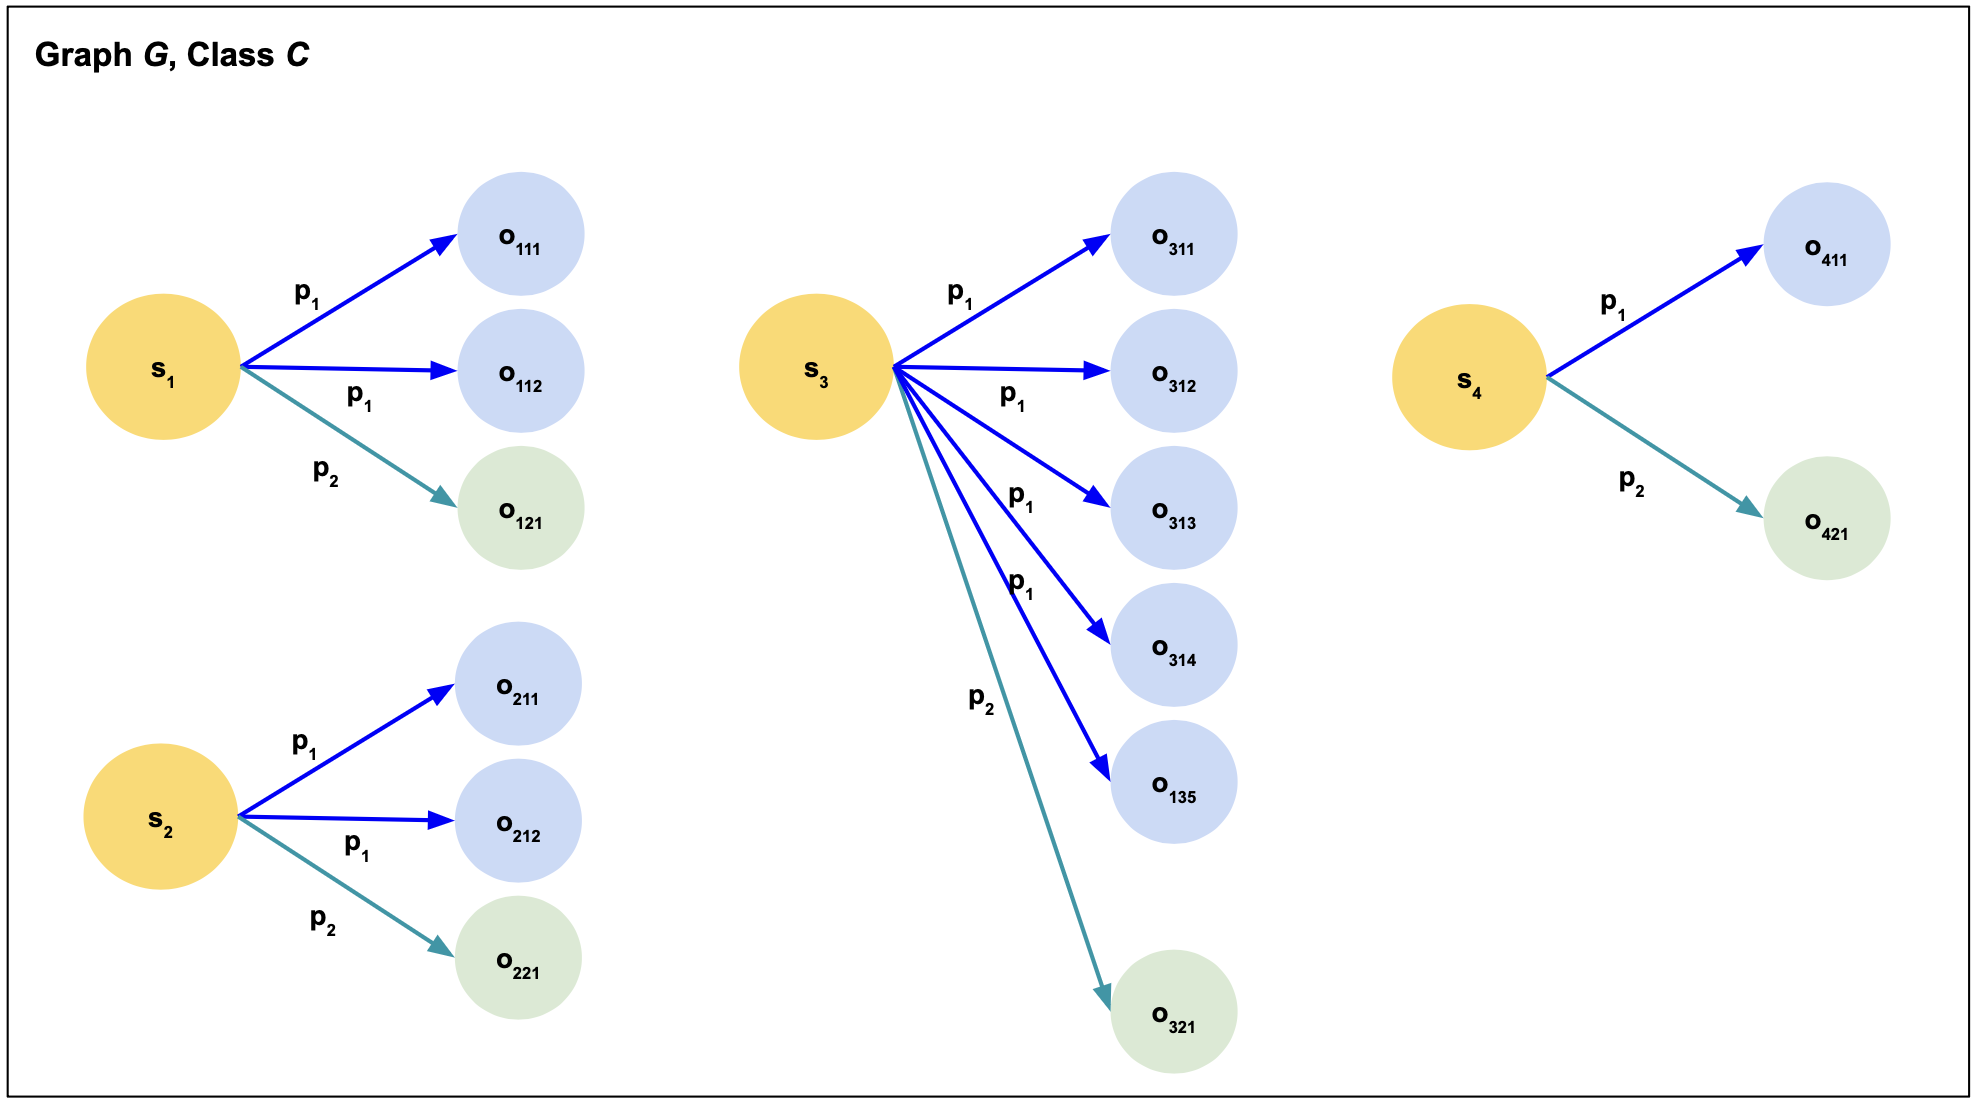
\includegraphics[scale=.3]{Wealth Weighted}
    \caption{Illustration of ...}
    \label{fig:wealth-weighted}
\end{figure}